\documentclass{article}

\usepackage{tikz} 

\usetikzlibrary{positioning} % Required for positioning of nodes

\begin{document}

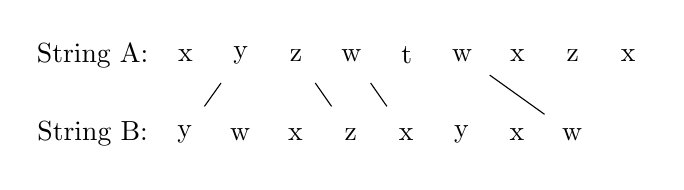
\begin{tikzpicture}[node distance = 0pt,
IdxStyle/.style={draw=none, minimum width=2em, minimum height=2em, 
                outer sep=0pt},]
\node [IdxStyle] at (0, 1) (u1) {String A:};
\node [IdxStyle, right=of u1] (u2) {x};
\node [IdxStyle, right=of u2] (u3) {y};
\node [IdxStyle, right=of u3] (u4) {z};
\node [IdxStyle, right=of u4] (u5) {w};
\node [IdxStyle, right=of u5] (u6) {t};
\node [IdxStyle, right=of u6] (u7) {w};
\node [IdxStyle, right=of u7] (u8) {x};
\node [IdxStyle, right=of u8] (u9) {z};
\node [IdxStyle, right=of u9] (u10) {x};
\node [IdxStyle] (l1) at (0, 0) {String B:};
\node [IdxStyle, right=of l1] (l2) {y};
\node [IdxStyle, right=of l2] (l3) {w};
\node [IdxStyle, right=of l3] (l4) {x};
\node [IdxStyle, right=of l4] (l5) {z};
\node [IdxStyle, right=of l5] (l6) {x};
\node [IdxStyle, right=of l6] (l7) {y};
\node [IdxStyle, right=of l7] (l8) {x};
\node [IdxStyle, right=of l8] (l9) {w};

\draw (u3)--(l2);
\draw (u4)--(l5);
\draw (u5)--(l6);
\draw (u7)--(l9);
\end{tikzpicture}

\end{document}